\section{System Model}\label{sec_system}
The system model consists of three parts: a software application, an execution platform, and a software allocation scheme. An overview of the system model is illustrated in Figure \ref{fig_softwareallocation}. The software application is a user-defined software system, such as x-by-wire, electronic throttle control, flight control, etc. that is developed using software components \cite{softwarecomponents}\cite{Crnkovic2002BuildingSystems}. The application is deployed on an execution platform, which is a network of heterogeneous nodes with possibly different processor frequencies, power consumption, and failure-rate. The allocation scheme, which defines a mapping relation from software components to computational nodes, guarantees that the extra-functional properties such as application reliability and timing requirements are met. Furthermore, it takes the optimization of power consumption as its objective in the allocation process.
\begin{figure}[!h]
\centering
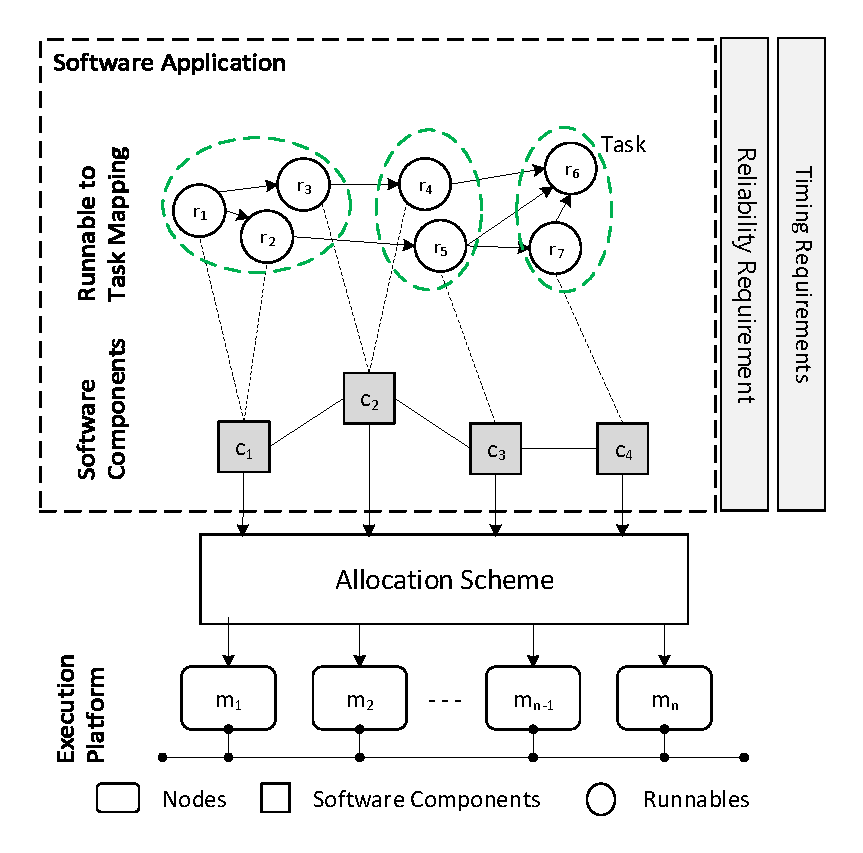
\includegraphics[scale=0.6]{softwareallocation}
\caption{Software Allocation Scheme.}
\label{fig_softwareallocation}
\end{figure}

In this work, we target AUTOSAR-based systems due the increasing popularity of specification standard in  the automotive industry, and the challenges and opportunities that automotive industries are facing especially in resource optimization and dependability of automotive systems. Note that our approach might also be applied on different distributed embedded systems with a slight change in the application modeling.

\subsection{Software Application Model}
In AUTOSAR-based systems, a software application is developed using AUTOSAR application software components that consist of one or more Runnables, which are atomic, shedulable piece of programs that are activated via events \cite{Schreiner2007ABus}.
\begin{definition}
Formally, we define an AUTOSAR software application $\zeta$ as a \textit{Digraph} (acyclic directed graph) $\langle V_r, E\rangle$ of Runnable nodes $V_r$, where $\langle u,v\rangle\in E$ is a set of directed links (or arcs) from $u$ to $v$ that denote the logical flow of the application. The runnable is associated with execution times $e=\{e_i=1,2,\dots N\}$ and a triggering mechanism, where $e_i$ refers to the execution time of a Runnable on node $n_i$. 
\end{definition}
 
Our proposed software allocation is based on the following assumptions:
\begin{itemize}
\item Atomicity of software components - allocatable software components are considered atomic and therefore are allocated only to a single node, and composite components need to be flattened first into their respective set of atomic component constituents.
\item Activation of Runnables - Runnables are activated either periodically by clock events or by predecessor Runnables that impose order of execution;
\item Runnables-to-Tasks mapping - three cases of mapping are considered in the allocation: i) Runnables-to-Task mapping - Runnables collocating on the same and have the same activation patters are mapped to a task; ii) Component-to-Task mapping - all Runnables collocated to a component are mapped to to a task; iii) Runnable-to-Task mapping - a Runnable is mapped to a task, inhering the execution time and period of the Runnable. For more of the various cases of Runnables-to-tasks mappings, we refer the reader to \cite{AUTOSAR2017SpecificationSoftware}.
\end{itemize}

\subsection{Fault-tolerant Software Application Model}
Redundancy is the most common way to increase the reliability of an application. It can be implemented according to different schemes, such as active replication, hot stand-by, cold stand-by, etc~\cite{Dubrova2013Fault-tolerantDesign}. In this work the details of the redundancy scheme are abstracted away under the following assumptions: i) Hot stand-by redundancy technique is used for the replication of components, which are identical and are allocated on different nodes. ii) Software components need to be replicated if the application's reliability requirement is not met without replication, otherwise they are not replicated. iii) The time needed to detect and replace a faulty component is considered negligible and will not be taken into account in the response time analysis of tasks and delay calculation of cause-effect chains. iv) Because of its simplicity, the mechanism for detection and replacement of faulty components will be considered fault-free and therefore will not be included in the reliability calculations.

We denote the $k^{th}$ replica of a software component $c$ as $c^k$, with $1\le k\leq K$; where $K$ is the maximum number of replicas allowed for each application component.

\subsection{Platform Model}
The application is deployed on a network of heterogeneous computing nodes that are connected via a reliable communication network, the CAN bus. A computational node is specified as a tuple $\langle hz, \lambda, p \rangle$, respectively for processor frequency, failure-rate and power consumption of a node. Due to the heterogeneity assumption of the processors, an application maybe be deployed on nodes with higher processor frequencies and fewer number of nodes in order to reduce the total power consumption. However, due to the application reliability constraint imposed on the system, the application could be deployed differently. Figure~\ref{fig_softwareallocation} illustrates an overview of an AUTOSAR software application deployment on a set of computational nodes via a software allocation scheme that is discussed in Section~\ref{sec_allocation}.

